\documentclass[a4paper]{article}
\usepackage{array}
\usepackage{algorithmicx}
\usepackage{algorithm}
\usepackage{algpseudocode}
\usepackage{tabu}
\usepackage{longtable}
\usepackage[table]{xcolor}
\usepackage{hyperref}
\usepackage{float}
\usepackage{wrapfig}
\usepackage{enumerate}
\usepackage{enumitem}
\usepackage[utf8]{inputenc}
\usepackage{graphicx}
\usepackage{pgfgantt}
\usepackage{amsmath}
\usepackage{tikz}
\usepackage[margin=1 in]{geometry}
\usepackage{color}
\usepackage{caption}
\usepackage{subcaption}
\usepackage[usenames,dvipsnames]{pstricks}
\usepackage{epsfig}
\usepackage{textcomp}
\definecolor{listinggray}{gray}{0.9}
\usepackage{listings}
\lstset{
	language=,
	literate=
		{æ}{{\ae}}1
		{ø}{{\o}}1
		{å}{{\aa}}1
		{Æ}{{\AE}}1
		{Ø}{{\O}}1
		{Å}{{\AA}}1,
	backgroundcolor=\color{white},
	tabsize=2,
  numbers=left,
	rulecolor=,
	basicstyle=\scriptsize,
	upquote=true,
	aboveskip={0.2\baselineskip},
	columns=fixed,
	showstringspaces=false,
	extendedchars=true,
	breaklines=true,
	prebreak =\raisebox{0ex}[0ex][0ex]{\ensuremath{\hookleftarrow}},
	frame=single,
	showtabs=false,
	showspaces=false,
	showlines=true,
	showstringspaces=false,
	identifierstyle=\ttfamily,
	keywordstyle=\color[rgb]{0,0,1},
	commentstyle=\color[rgb]{0.133,0.545,0.133},
	stringstyle=\color[rgb]{0.627,0.126,0.941},
  moredelim=**[is][\color{blue}]{@}{@},
}

\lstdefinestyle{base}{
  emptylines=1,
  breaklines=true,
  basicstyle=\ttfamily\color{black},
}

\definecolor{barblue}{RGB}{153,204,254}
\definecolor{groupblue}{RGB}{51,102,254}
\definecolor{linkred}{RGB}{165,0,33}
\def\x{\mbox{\textbf{x}}}
\def\w{\mbox{\textbf{w}}}
\def\Pr{\mbox{\textbf{Pr}}}
\def\qvec#1#2{\begin{bmatrix} #1 \\ #2 \end{bmatrix}}
\makeatletter
\renewcommand{\ALG@beginalgorithmic}{\footnotesize}
\makeatother
\usetikzlibrary{shapes}
\title{Needleman-Wunsch using OpenMP and MPI\\Parallel and Multicore Programming\\COMP 90025\\Project 2}
\author{Matthieu Bergeron - 849438\\Tobias Hallundbæk Petersen - 845234}
\begin{document}
\maketitle
\section{Introduction}
The Needleman-Wunch (NW) algorithm is designed for and used to align sequences in within bioinformatics. It is very closely related to the Smith-Waterman algorithm for local sequence alignment, and they share the approach of solving their respective problems by using dynamic programming. In this report, the NW algortihm will be optimized to work in a multiprocessor environment, this will be done using the two parallelization APIs: openMP and MPI.

\section{Methods}
Although two different parallel programming APIs are used in this report, the method used to solve the problem is the same. This method will be explained and analysed to determine its theoretical effectiveness.
\subsection{Idea}
The NW algorithm works by populating a matrix from the north-western corner towards the south-eastern corner. Which in practicality means that, to determine the value of any number in the matrix, the western, northern and north-western value needs to be computed first.

So the work needs to be partitioned in a non-trivial way to maximize the processor power used in a multiprocessor environment.

A tiling approach was here explored\footnote{http://www.ijascse.org/volume-3-issue-6/OpenMp.pdf}, with the thought being to divide the computation matrix into a number of tiles, the power of these tiles is that we can decide their size, and thus optimize it to the given cache size of the multiprocesssor environment we are working in.

Another power of these tiles is that, as individual values, a tile can be calculated if the western, southern and south-western tile has been computed This leads us to the order in which these tiles will be computed, which is described in Figure \ref{fig2}. Every diagonal strip of tiles will be able to be computed concurrently, which means that for a large enough amount of tiles, the amount of processors that can be active will be incremented by one for every strip, until the strips narrow down in size.
\begin{figure}[H]
  \center
  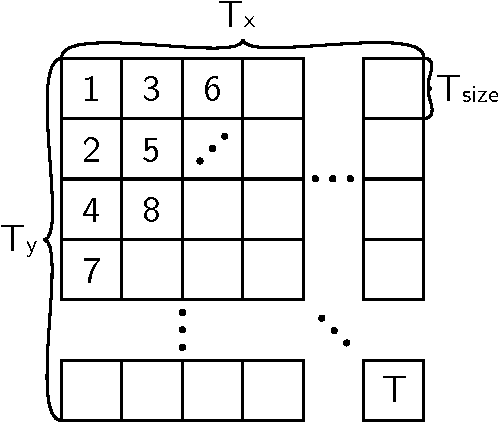
\includegraphics[width=0.4\textwidth]{fig/fig2.pdf}
  \caption{The ordering the tiles are computed in.}
  \label{fig2}
\end{figure}
Every tile will be responsible for computing three things, its southern edge, eastern edge and the south-eastern corner, which it will be able to feed to its respective neighbouring tiles. This input-output relationship is shown in Figure \ref{fig1}, this figure also shows the input corner, which is always 0, and it output corner, which is the final output of the algorithm.
\begin{figure}[H]
  \center
  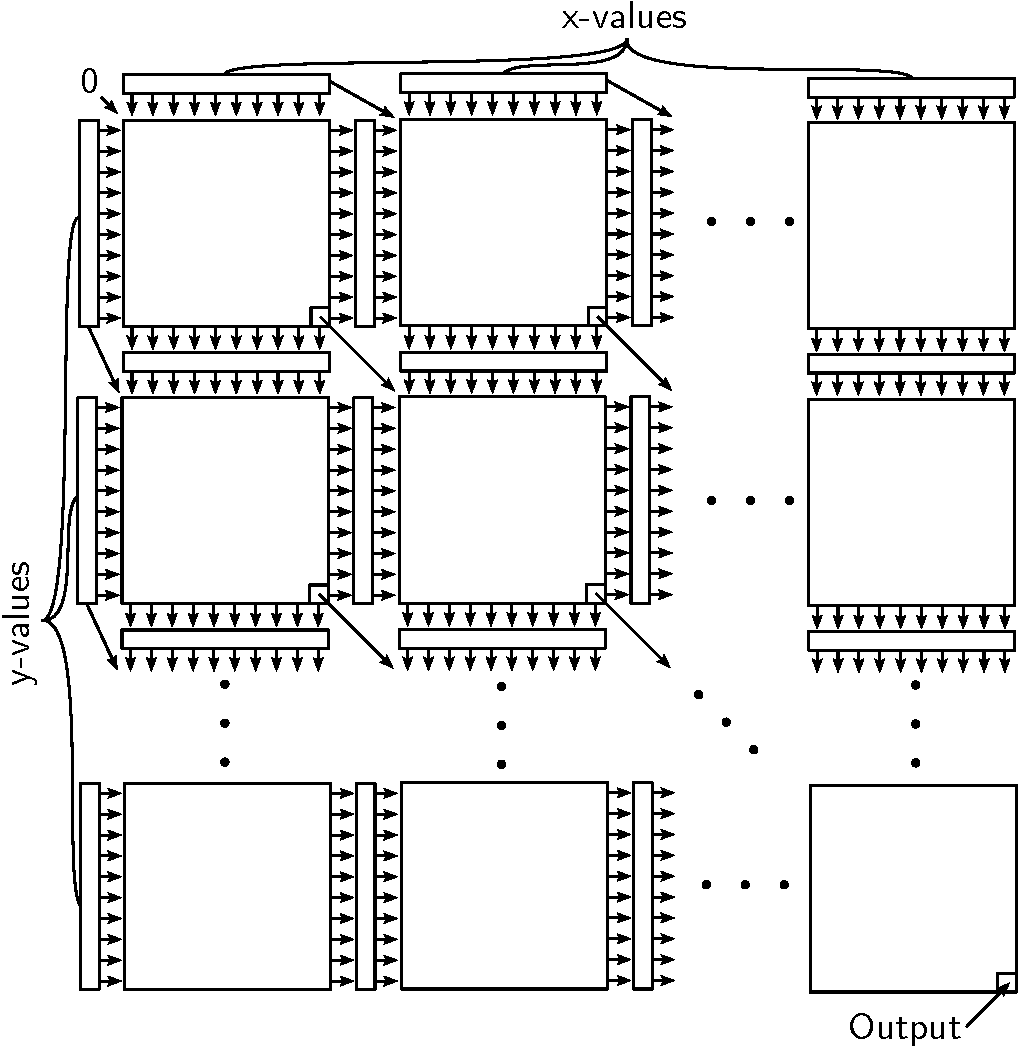
\includegraphics[width=0.7\textwidth]{fig/fig1.pdf}
  \caption{The input and output of the tiling structure. Each tile here will populate their western and northern edges using their input arrays and input corner, their output will be their eastern and southern edges and their south-eastern corner.}
  \label{fig1}
\end{figure}
The way this is structured ensures there is only a memory usage of $p\cdot T_{size}^2$, where $p$ is the amount of processors, and $T_{size}$ is the length of a tiles side, which is important in dealing with large inputs, as the entire solution matrix is never in memory at the same time. The also implies that the solution to reach the best alignment, is lost, only the final score is reported.

\subsection{Analysis}
For the analysis, the input string are assumed to be of the same length, and divisible by the tile size $T_{size}$, this means that relative to the definitions in Figure \ref{fig2}, that $T_x^2 = T_y^2 = T$, and that $T_x \% T_{size} = 0$, where $\%$ is the modulo operator. The amount of processors is here denoted $p$, thus for the first $p$ diagonal strips we will have the following procssor usage
$$
\frac{\sum_{i=1}^p i}{p^2} = \frac{p+1}{2p}
$$
This is going to be happening twice, once when the strips are increasing in size, and once at the end where they are decreasing.Which means that there will be a total processor usage at the corners of
$$
\frac{p+1}{2p}
$$
For the middle part all processors will be active, to understand how big this part is compared to the beginning and end, the amount of tiles in this part is calculated to
$$
  T - p(p+1).
$$
In these tiles the processor usage will be maximized, which means that the total processor usage will be
$$
\frac{T - p(p+1) + p(p+1)\frac{p+1}{2p}}{T}
$$
The processor usage will be directly related to the speedup, which will be
$$
p \left(\frac{T - p(p+1) + p(p+1)\frac{p+1}{2p}}{T}\right) = \frac{p - p^3}{2T} + p
$$
This will only hold if there is a middle part, which is in cases where $T - p(p+1) > 0$, for values appropriate the speedup can be calculated for different values which is shown in Table \ref{tab1}.
\begin{table}[H]
  \center
  \begin{tabular}{|c||c|c|c|c|}
  \hline
          & \multicolumn{4}{c|}{Processors ($p$)}\\
  \hline
     T    & 4    & 8     & 16    & 32\\
  \hline
     64   & 3.53 & 4.06  & -     & - \\
  \hline
     256  & 3.88 & 7.02  & 8.03  & - \\
  \hline
     1024 & 3.97 & 7.75  & 14.01 & 16.02 \\
  \hline
     4096 & 3.99 & 7.94  & 15.50 & 28.00\\
  \hline
  \end{tabular}
  \caption{Theoretical speedup relative to amount of tiles $T$ and processors $p$.}
  \label{tab1}
\end{table}

\section{Implementation}
In this section, the implementation specifics of the OpenMP and MPI soloution is explained. The main focus of this is to explain the difference in the two.
\subsection{OpenMP}
The implementation was somewhat straightforward with OpenMP, implementing it the way that was described in the method section, the only thing left to do was parallelizing the strips, as all tiles in each strip can be calculated concurrently.

The code was written such that the loop iterating over the strips is for-loop, which is ideal for OpenMP, as the line
\begin{lstlisting}
#pragma omp parallel for
\end{lstlisting}
Will enable the iterations of a for loop to run concurrently. And as there is no inter-data dependency within each strip, this is the preferred implementation. The only thing to keep in mind is the variables which should be shared, and which should be private.

\subsection{MPI}
The MPI implementation of the Needleman-Wunsch algorithm uses a Master-Slave paradigm. \\
The master process is in charge of distributing the jobs to the slaves processes. However, the job scheduling is not dynamic : for each diagonal, the master distributes the jobs according to the same pattern. For pratical purposes, the master thread is computing the first tile.
\begin{figure}[htp]
\centering
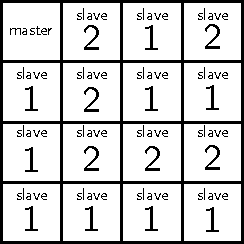
\includegraphics[scale=1.00]{/home/matthieu/Documents/melbourne/cours/parallel_prog/git/nw_parallel/report/fig/mpi1.pdf}
\caption{Scheduling for -np 3 (2 slaves and 1 master)}
\label{}
\end{figure}
\\
One of drawbacks of this technique is that some slaves processes can be waiting for others. But since the tile size is the same for every slave, the workload should be similar among slaves. \\

\section{Results}
The two implementations along with the sequential implementation will be tested with varying parameters, these parameters will first be explained, followed by the actual results.
\subsection{Methods}

In the benchmarks results above, we focus on two paramers : the tile size and the numbers of processors. \\
For the openMP algorithm, we make use of one single node, and scale the numbers of processors from 2 to 16. \\
The MPI algorithm is run with 2,4,8 or 16 nodes, depending on the numbers of processors required. \\
All the results have been computed on the VLSCI Avoca server. It's important to note that our results have a lot of variance. During experimentations, we observed differents running time for the same parameters and inputs. The Avoca server can have performances that range from a scale of 1 to 10 (for instance : a program that runs in 0.7 seconds one day can run in 7s another day).\\
In order to have an idea of the performances of our parallel implementations, we have run a sequential algorithm on the same benchmark. \textbf{The timing of the sequential algorithm is 9.8s}.
\\
The benchmark is composed of two random sequences of size $2^{15}$.
\subsection{Benchmarks}
T denotes the size of one side of a tile.
\subsection{OpenMP}
Running times : \\ \\
\begin{center}\begin{tabular}{|l||l|l|l|l|}
\hline
	& \multicolumn{4}{c|}{Processors ($p$)} \\
\hline
	T & 2 & 4 & 8 & 16\\
\hline
	128 & 5,6s & 2,85s & 1,74s & \textbf{1,2s}\\
\hline
	256 & 5,7s & 2,885s & 1,69s & 1,28s\\
\hline
	512 & 5,63s & 3,277s & 1,76s & 1,36s\\
\hline
	1024 & 5,72s & 3s & 1,99s & 1,55s\\
\hline
\end{tabular}\end{center}
\newpage
Here is the results in terms of speed-up in order to compare with the analysis : \\ \\
\begin{center}\begin{tabular}{|l||l|l|l|l|}
\hline
	& \multicolumn{4}{c|}{Processors ($p$)} \\
\hline
	T & 2 & 4 & 8 & 16\\
\hline
	128 & 1,75 & 3,43 &  5,63 &\textbf{8,16}\\
\hline
	256 & 1,71 & 3,37 & 5,8 & 7,65\\
\hline
	512 & 1,74 & 2,98 & 5,56 & 7.2\\
\hline
	1024 & 1,71 & 3,26 & 4,92 & 6,32\\
\hline
\end{tabular}
\end{center}
\subsection{MPI}
Running times : \\ \\
\begin{center}\begin{tabular}{|l||l|l|l|l|l|l|l|l|}
\hline
	& \multicolumn{4}{c|}{Processors ($p$)}\\
\hline
	T & 2 & 4 & 8 & 16 & 32 & 64 & 128 & 256\\
\hline
	128 & 1m13s & 29,4s & 15,35s & 8,16s & 6s & 5,66s & 5,11s & 5,6s\\
\hline
	256 & 1m10s & 26s & 44 & 13,85s & 7,04s & \textbf{5s} & 5,33s & 5,46s\\
\hline
	512 & 1m08s & 25,8s & 54 & 13,73s & 7,2s & 6,29s & 6,18s & 6,19s\\
\hline
	1024 & 1m08s & 26,4s & 64 & 14,6 & 8,1s & 8,13s & 8,08s & 8,15s\\
\hline
\end{tabular}
\end{center}
\section{Discussion}
There are two main focuses of this section, the first being how well our implementation compares to the theoretical analysis. The second being a comparison of the two different APIs, and what could have affected the difference.
\subsection{Comparison to Analysis}
The openMP results are quite close to the analysis. Indeed, the speed-up scores for a given number of cpus are comparable with the results found in part (3.2). \\
 The tile size does not seems to have such a great impact on the performances of both openMP and MPI versions of the algorithm. However, it is important to note that running the algorithm with a tile size lower than 64 gives poors performance. We have not included the results here because the program is running out of memory when the tile size is too little. \\
The performances of the MPI algorithm are way lower than what we could expect from the theoritical analysis. We will discuss this in the next part.
\subsection{OpenMP vs. MPI}
The openMP version of the algorithm is clearly faster than the MPI one. \\ This is due to the low granularity of the MPI algorithm. Indeed, a large amount of data is send between processes during the algorithm :  \\
- Every slave sends an array of $TILESIZE*sizeof(int)$ to the master process after computing its own tile.  \\
- Since all these sendings can't occur at the same time, slaves processes can spend a lot of time waiting to send their results.\\ \\ \\
However, the MPI algorithm can compete with the openMP one for very large numbers of CPUS. For longer sequences, it could be possible that the MPI algorithms runs faster than the openMP one; however we would have to use an extremely high number of processors (maybe more than 64 !) .\\

To conclude, due to the low granularity of the problem it seems better to implement the Needleman-Wunsch algorithm with openMP.
\end{document}
